\documentclass{article}

%% Language and font encodings
\usepackage[english]{babel}
\usepackage[utf8x]{inputenc}
\usepackage[T1]{fontenc}
\usepackage{amsfonts}
\usepackage[margin=41mm]{geometry}
\usepackage{mathtools}

%% Sets page size and margins
%\usepackage[a4paper,top=3cm,bottom=2cm,left=3cm,right=3cm,marginparwidth=1.75cm]{geometry}

%% Useful packages
\usepackage[colorlinks=true, allcolors=black]{hyperref}
\usepackage{amsmath}
\usepackage{xcolor}
\usepackage{amssymb}
\usepackage{amsthm}
\usepackage{stmaryrd}
\usepackage{graphicx}
\usepackage{enumitem}
\usepackage{tikz, tkz-euclide}
\usetikzlibrary{positioning}
\usepackage{tikz-cd}

%Theorem
\theoremstyle{plain}
\newtheorem{theorem}{Theorem}[subsection]
\newtheorem{proposition}[theorem]{Proposition}
\newtheorem{lemma}[theorem]{Lemma}
\newtheorem*{corollary}{Corollary}
\newtheorem*{theorem*}{Theorem}
\theoremstyle{definition}
\newtheorem*{definition}{Definition}

\newtheorem{innercustomthm}{Proposition}
\newenvironment{customthm}[1]
  {\renewcommand\theinnercustomthm{#1}\innercustomthm}
  {\endinnercustomthm}

%Usual Sets
\newcommand{\C}{\mathbb{C}}
\newcommand{\R}{\mathbb{R}}
\newcommand{\Q}{\mathbb{Q}}
\newcommand{\Z}{\mathbb{Z}}
\newcommand{\N}{\mathbb{N}}
\newcommand{\F}{\mathbb{F}}
\newcommand{\E}{\mathbb{E}}
\newcommand{\K}{\mathbb{K}}
\newcommand{\Zn}[1]{\mathbb{Z}/ #1 \mathbb{Z}}

%Categories
\newcommand{\CatC}{\textbf{C}}
\newcommand{\CatD}{\textbf{D}}
\newcommand{\CatTop}{\textbf{Top}}
\newcommand{\CatSets}{\textbf{Sets}}
\newcommand{\CatGps}{\textbf{Gps}}
\newcommand{\CatAbGps}{\textbf{AbGps}}
\newcommand{\CatMod}[1]{_\textbf{#1}\textbf{Mod}}
\newcommand{\CatVect}[1]{_\textbf{#1}\textbf{VSp}}

%Special Sets
\newcommand{\Iint}[2]{\llbracket #1 , #2 \rrbracket}

%Math Operators
\let\Re\relax
\let\Im\relax
\DeclareMathOperator{\Im}{Im}
\DeclareMathOperator{\Re}{Re}
\DeclareMathOperator{\Null}{null}
\DeclareMathOperator{\range}{range}
\DeclareMathOperator{\card}{card}
\DeclareMathOperator{\Aut}{Aut}
\DeclareMathOperator{\Hom}{Hom}
\DeclareMathOperator{\Mor}{Mor}
\DeclareMathOperator{\Gal}{Gal}
\DeclareMathOperator{\Char}{char}

%Others
\newcommand{\td}{\textcolor{red}{\textbf{TODO}}}
\newcommand{\isomorphic}{\cong}

\title{MATH 338 Tutorials : Constructible Numbers}
\author{Samy Lahlou}
\date{}

\begin{document}

\maketitle

\section*{Introduction}

The goal of this short document is to motivate and explain the notion of constructible numbers. This is an important notion because it helps understanding and solving a lot of ancient problems in Euclidean Geometry, more precisely, straightedge and compass constructions (which is at the heart of the first five chapters of the course).

Before diving into constructible numbers, let's first recall what we can and cannot do with a straithedge and a compass on the plane. To do this, we will rely on the set of five axioms that Euclid stated at the beginning of the Book I of his \textit{Elements}:

\begin{enumerate}[label=\textbf{A\arabic*.}]
    \item It is possible to draw a straight line from any point to any point.
    \item It is possible to produce a finite straight line continuously in a straight line.
    \item It is possible to describe a circle with any circleand distance (i.e., radius)
    \item All right angles are equal to one another.
    \item If a straight line falling on two straight lines make the interior angles on the same sides less than two right angles, the two straight lines, if produced indefinitely, meet on that side on which are the angles less than the two right angles.
\end{enumerate}

From these five axioms and some common notions, Euclid was able to deduce a lot of propositions that will be very useful for the next section. I will try to state most of them but it would take too much time to prove all of them:

\begin{customthm}{I.3}\label{1.3}
    \textit{Given two unequal straight lines, [it is possible] to cut off from the greater a straight line equal to the less.}
\end{customthm}

This proposition simply states that given a segment $AB$, a line $L$ and a point $C$ on $L$, it is possible to construct the point $D$ on $L$ such that $AB = CD$ (\autoref*{fig:Prop1.3}). Propositions I.10 and I.11 are already clear from their statements.

\begin{figure}[h!]
    \centering
    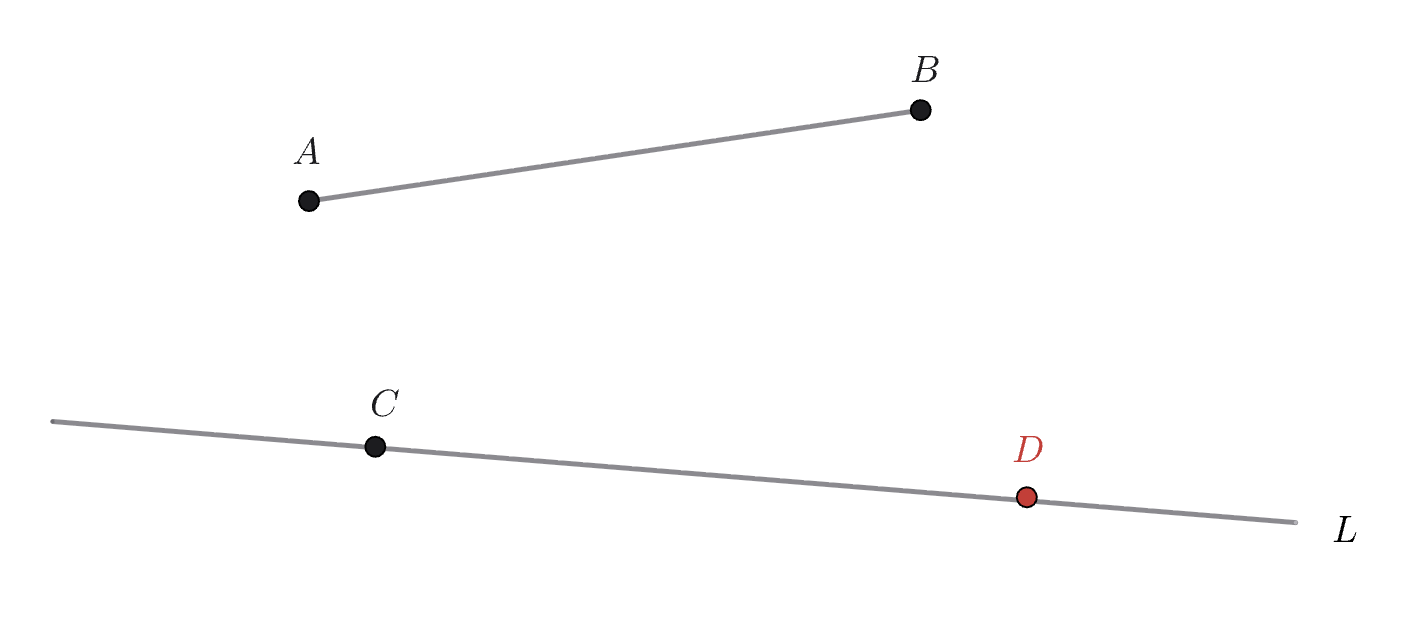
\includegraphics[scale=0.35]{pics/Prop1.3.png}
    \caption{Proposition I.3}
    \label{fig:Prop1.3}
\end{figure}

\begin{customthm}{I.10}\label{1.10}
    \textit{[It is possible] to bisect a given finite straight line.}
\end{customthm}

\begin{customthm}{I.11}\label{1.11}
    \textit{[It is possible] to draw a straight line at right angles to a given straight line from a given point on it.}
\end{customthm}

The following proposition is a generalization of Thales' Theorem (Figure 2).

\begin{customthm}{III.20}\label{3.20}
    \textit{In a circle the angle at the centre is double of the angle at the circumference, when the angles have the same circumference base.}
\end{customthm}

\begin{corollary}[Thales' Theorem]
    In a circle, the angle on the circumference of a triangle which has a side equal to the diameter is always a right angle.
\end{corollary}

\begin{figure}[h!]
    \centering
    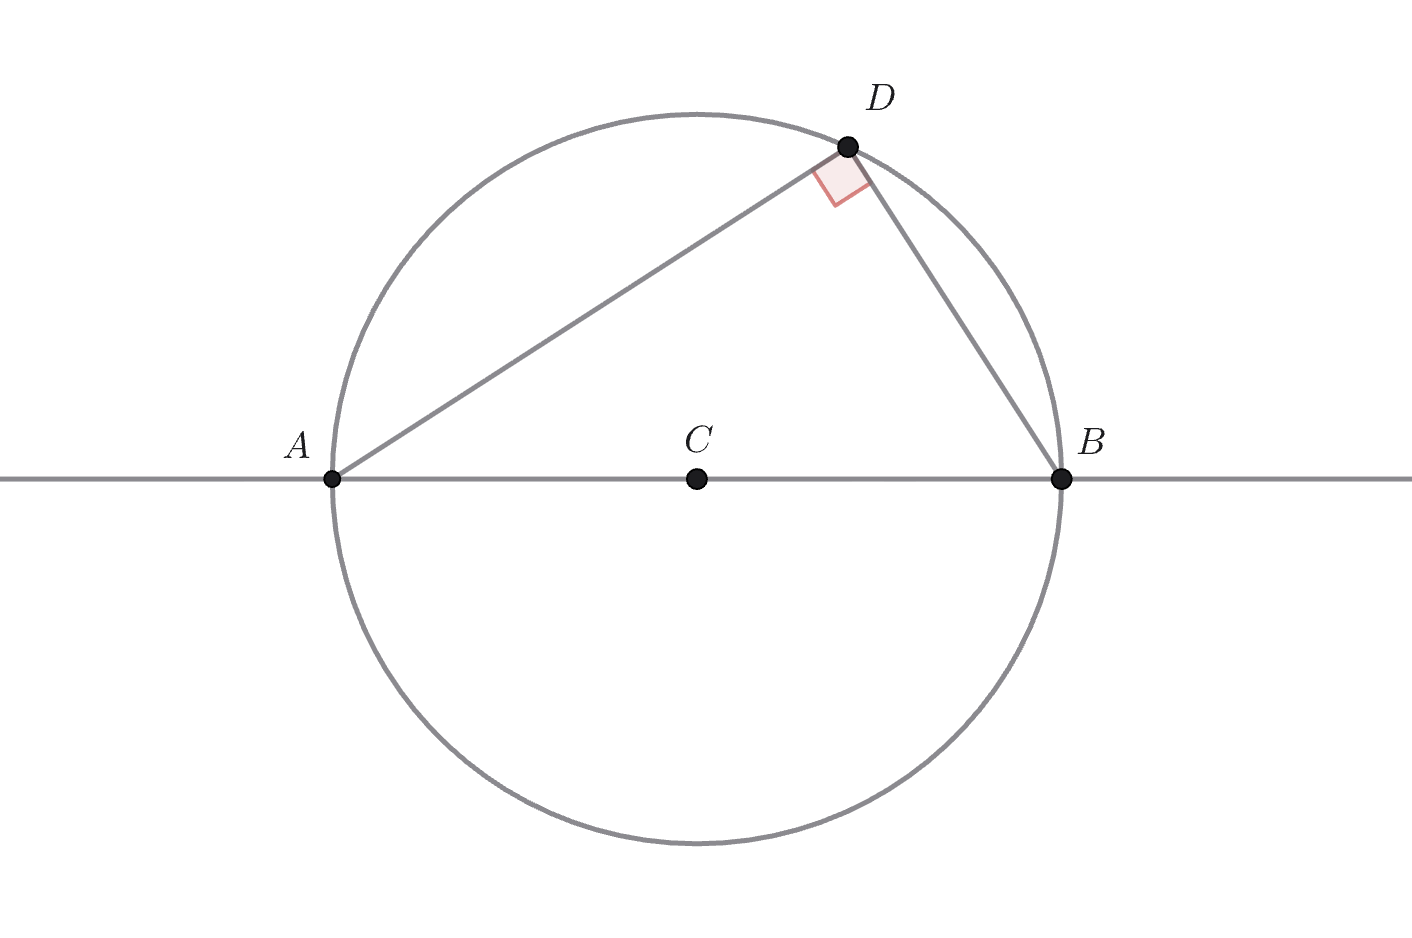
\includegraphics[scale=0.34]{pics/Thales Theorem.png}
    \caption{Thales' Theorem}
\end{figure}

The following and last proposition that we will need is Proposition VI.4.

\begin{customthm}{VI.4}\label{6.4}
    \textit{In equiangular triangles the sides about the equal angles are pro-portional, and those are corresponding sides which subtend the equal angles.}
\end{customthm}

In other words, it states that if two triangles avec the same angles (Figure 3), then we have the following ratios:
$$\frac{AB}{DE} = \frac{BC}{EF} = \frac{AC}{DF}.$$

\begin{figure}[h!]
    \centering
    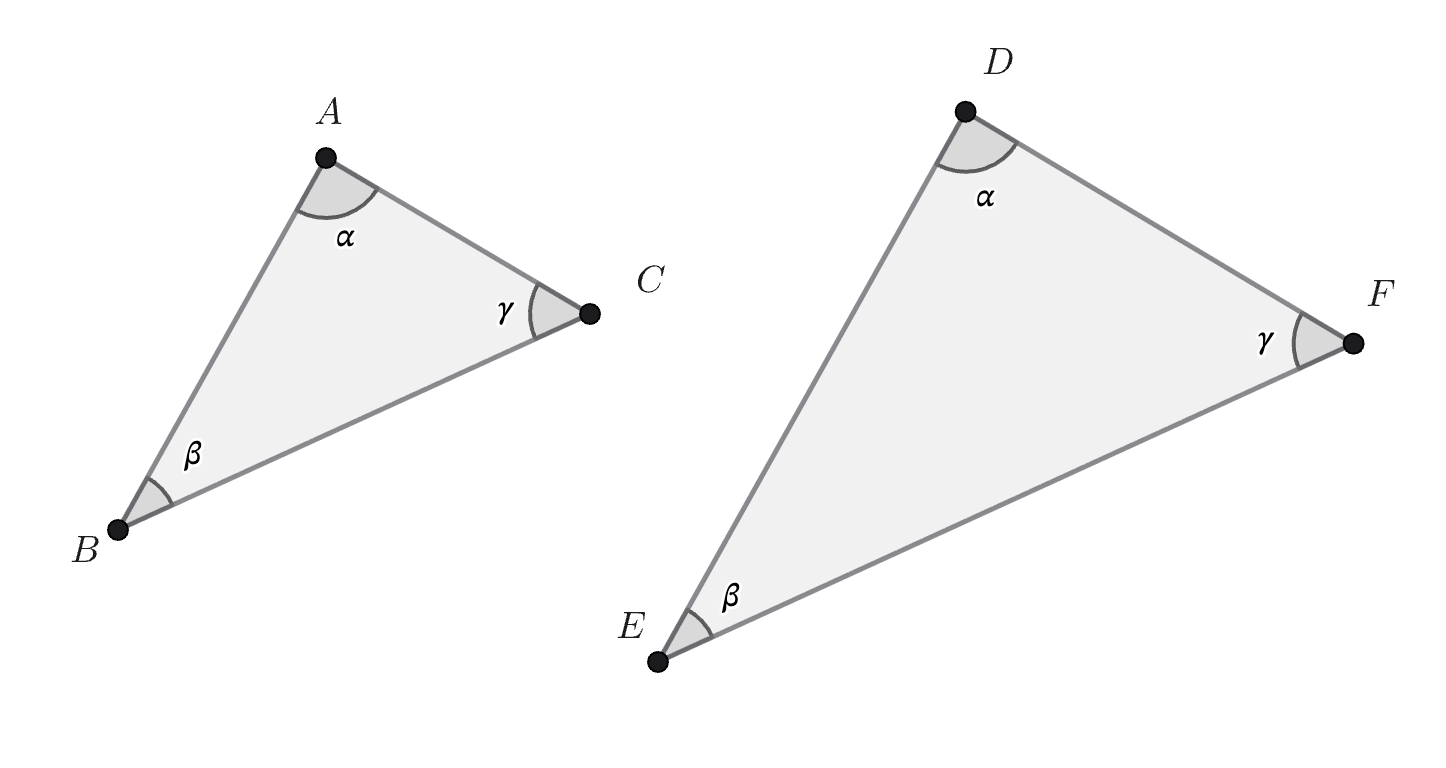
\includegraphics[scale=0.42]{pics/Prop6.4.png}
    \caption{Proposition VI.4}
\end{figure}

The proofs of these propositions can be found in the \textit{Elements}. It is a good exercise to try to follow the proof or to find yours. We are now ready to talk about constructibility.

\section*{Definition}

To define the notion of constructibility, let's recall that in Euclidean Geometry, we cannot measure lengths, this comes from the fact that we can only use a straight edge which is exactly the same as an unmarked ruler. However, we can compare lengths. For example, if we are given a segment $AB$ in which we construct the midpoint $C$, then we can say that the length of $AB$ is twice the length of $AC$ or $BC$. This shows that even though there is no general way of saying that a segment is short or long, there is however a way of saying that a given segment is short or long if it is compared to another. Therefore, we can take an arbitrary segment $AB$ and define the length of 1 as the lengh of $AB$, and then compare the length of every other segment to $AB$ to deduce the length of the other segments. In that case, we call $AB$ the \textit{unit segment}. For example, if we let a segment $AB$ be the unit segment, then the length of $AC$ is $1/2$ where $C$ is the midpoint of $AB$. This motivates the following definition:

\begin{definition}
    A number $x$ is said to be constructible if, given a unit segment, it is possible to construct a segment of length $x$.
\end{definition}

\noindent It is clear from this definition that we can only construct positive numbers. The example above shows that $1/2$ is a constructible number. In the same way, it is possible to construct other numbers. For example, in the following construction (Figure 4), we have that $2$ is constructible because the segment $AB$ has length 1 and the segment $BC$ also has length 1, it follows that $AC$ has length 2. Thus, $2$ is constructible.

\begin{figure}[h!]
    \centering
    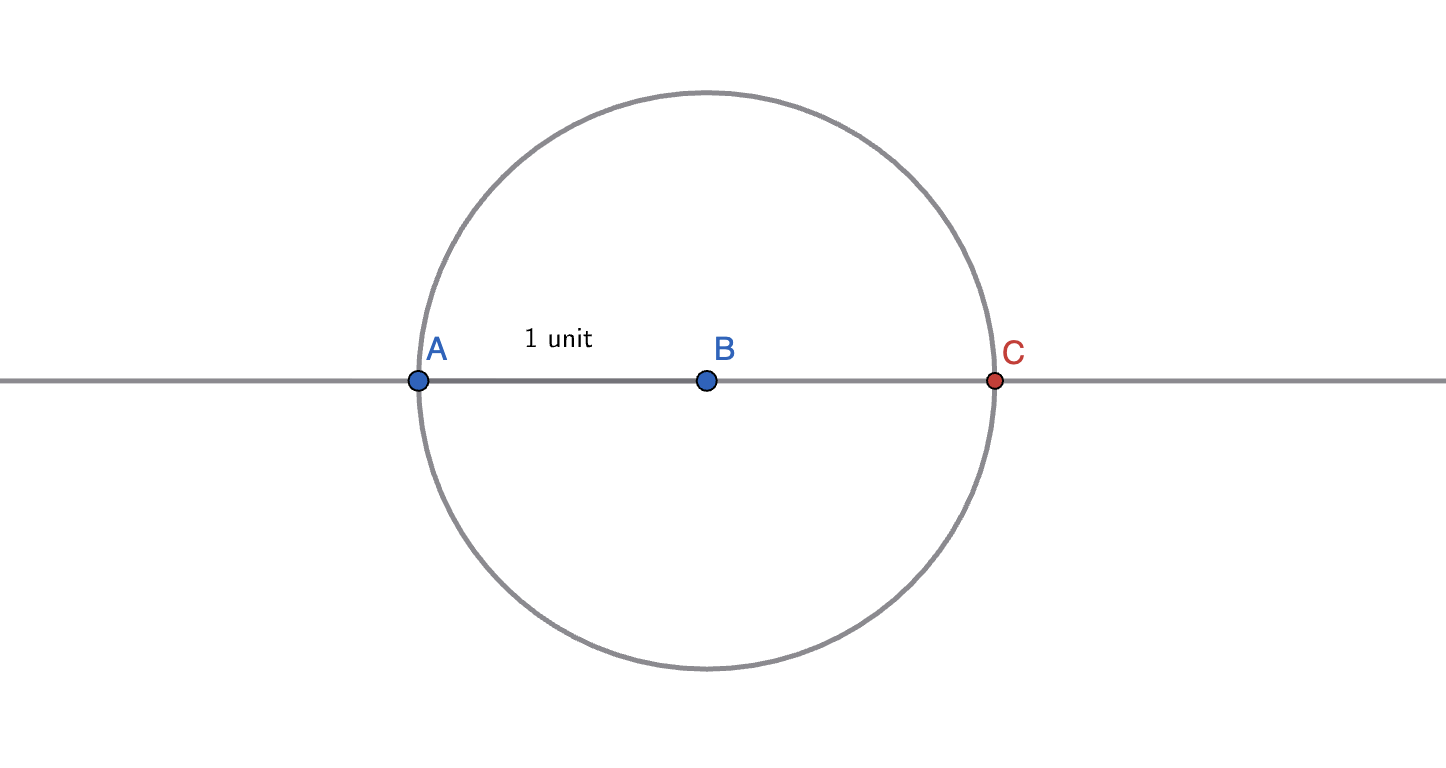
\includegraphics[scale=0.35]{pics/2construct.png}
    \caption{2 is constructible}
\end{figure}

If we repeat this process, we get that every positive integer is constructible (something that we will prove later). Moreover, these are not the only constructible numbers because we saw above that $1/2$ is also constructible. What about other positive fractions ? Can every positive fraction be constructible ? What about positive irrational numbers ? Concerning irrational numbers, it is actually easy to show that at least one of them is constructible. This comes from the fact that given the unit segment $AB$, we can construct a square of side length 1 and hence, construct the diagonal which has length $\sqrt{2}$. It follows that $\sqrt{2}$ (an irrational number) is constructible. We are now left with the following questions: which numbers are constructible ? Are every positive real numbers constructible ? The goal of the next sections is to answer these last two questions.

\section*{Operations on Constructible Numbers}

Throughout this section, we will fix a segment $AB$ and define it as the unit segment. When the segment $AB$ will be mentioned in this section, it referes to the unit segment. Let's prove some useful properties of constructible numbers that will let us determine easily which numbers are constructible.

\begin{customthm}{A}\label{A}
    \textit{If $x$ and $y$ are two constructible numbers, then $x + y$ is also constructible. Moreover, if $x$ is greater than $y$, then $x - y$ is also constructible.}
\end{customthm}

\begin{proof}
    Suppose that we are given segments $CD$ and $EF$ of length $x$ and $y$ respectively (Figure 5), then by the second axiom (\textbf{A2}), we can construct the straight line $L$ as the extension of $CD$. Applying Proposition I.3 twice lets us construct the points $G$ and $H$ on $L$ such that the segment $DG = DH = EF = y$. It follows that the segment $CG$ has length $x + y$. Therefore, $x + y$ is constructible. If $x > y$, then $CH$ has length $x - y$ and so $x - y$ is also constructible.
\end{proof}

\begin{figure}[h!]
    \centering
    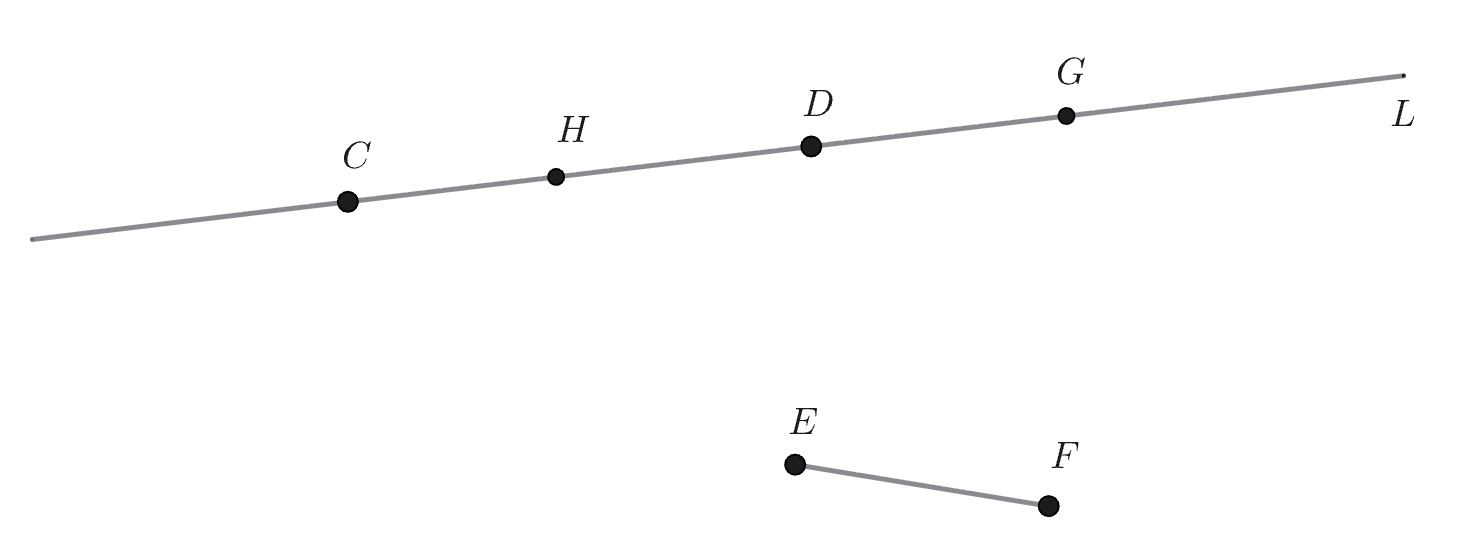
\includegraphics[scale=0.3]{pics/PropositionA.png}
    \caption{Proposition A}
\end{figure}

\noindent As a direct corollary, we have the following proposition:

\begin{corollary}
    Every positive integer is constructible.
\end{corollary}

\begin{proof}
    Since the segment $AB$ is given and has length 1 by definition, then it directly follows that 1 is constructible. By Proposition A, since 1 is constructible, then $2 = 1+1$ is constructible. Again, by the same proposition, since $1$ and $2$ are constructible, then $3 = 1 + 2$ is constructible. We can convince ourselves that this process can be used to generate every other positive integer. A more rigorous proof can be done by induction.
\end{proof}

Thus, we have proved that the sum of two constructible number is also a constructible number. In other words, constructible numbers are closed under addition. It turns out that they are also closed under multiplication.

\begin{customthm}{B}\label{B}
    \textit{If $x$ and $y$ are two constructible numbers, then $xy$ is also constructible.}
\end{customthm}

\begin{proof}
    Suppose that we are given segments $CD$ and $EF$ of length $x$ and $y$ respectively (Figure 6). First, extend the segment $EF$ into the straight line $L_1$ (Axiom 2). Construct the point $G$ on the segment $EF$ such that $EG = AB = 1$ (Proposition I.3), and from $G$, construct the straight line $L_2$ which is perpendicular to $L_1$ (Proposition I.11). Similarly, construct the straight line $L_3$ that is perpendicular to $L_1$ and that passes through $F$ (Proposition I.11). Next, construct the point $H$ on $L_2$ such that $GH = CD$ (Proposition I.3), and use it to construct the straight line $L_4$ that passes through $E$ and $H$ (Axiom 1). To finish the construction, define the point $I$ as the intersection between $L_3$ and $L_4$. 

    Let's now prove that $IF$ has length $xy$. To do so, notice that the triangles $EGH$ and $EFI$ have all their angles equal. Hence, from Proposition VI.4, we have the following relation:
    $$\frac{IF}{GH} = \frac{EF}{EG}.$$
    Now, recall that $GH = CD = x$, $EF = y$ and $EG = AB = 1$. Hence, we can rewrite the previous relation as
    $$\frac{IF}{x} = \frac{y}{1}.$$
    and so $IF = xy$. Therefore, the number $xy$ is constructible.
\end{proof}

\begin{figure}[h!]
    \centering
    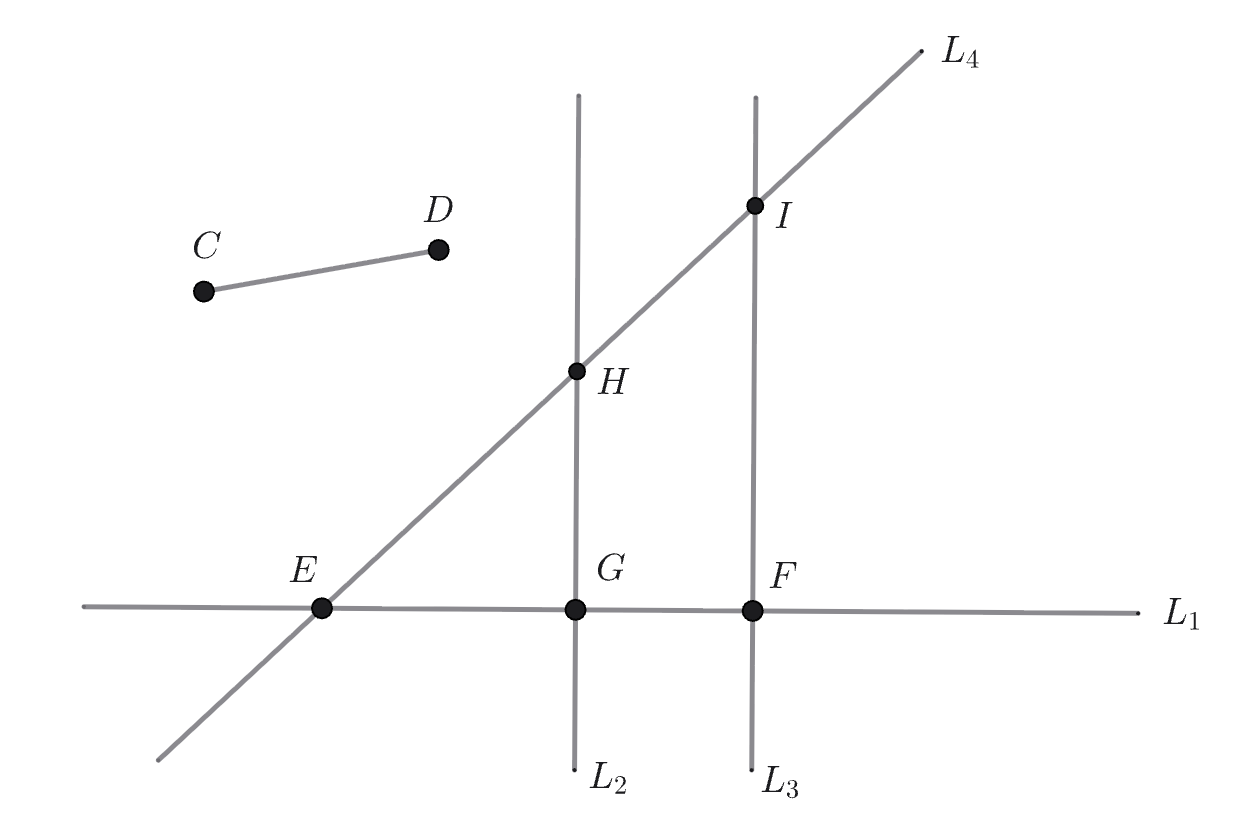
\includegraphics[scale=0.4]{pics/PropB.png}
    \caption{Proposition B and C}
\end{figure}

Proposition B is not very useful for the moment because it doesn't let us construct any more numbers than the positive integers (the multiplication of two positive integers is still a positive integer). However, we cannot say the same about the next proposition.

\begin{customthm}{C}\label{C}
    \textit{If $x$ and $y$ are two constructible numbers, then $x/y$ is also constructible.}
\end{customthm}

\begin{proof}
    The proof of this proposition is so similar to the previous one that we will use the same diagram (Figure 6). Suppose that we are given segments $CD$ and $EF$ of length $x$ and $y$ respectively. First, extend the segment $EF$ into the straight line $L_1$ (Axiom 2). Construct the point $G$ on the segment $EF$ such that $EG = AB$ (Proposition I.3), and from $G$, construct the straight line $L_2$ which is perpendicular to $L_1$ (Proposition I.11). Similarly, construct the straight line $L_3$ that is perpendicular to $L_1$ and that passes through $F$ (Proposition I.11). Next, construct the point $I$ on $L_3$ such that $IF = CD$ (Proposition I.3), and use it to construct the straight line $L_4$ that passes through $E$ and $I$ (Axiom 1). To finish the construction, define the point $H$ as the intersection between $L_2$ and $L_4$. 

    Let's now prove that $GH$ has length $x/y$. To do so, notice that the triangles $EGH$ and $EFI$ have all their angles equal. Hence, from Proposition VI.4, we have the following relation:
    $$\frac{IF}{GH} = \frac{EF}{EG}.$$
    Now, recall that $IF = CD = x$, $EF = y$ and $EG = AB = 1$. Hence, we can rewrite the previous relation as
    $$\frac{x}{GH} = \frac{y}{1}.$$
    and so $GH = x/y$. Therefore, the number $x/y$ is constructible.
\end{proof}

We are now able to deduce an important corollary.

\begin{corollary}
    Every positive rational number is constructible.
\end{corollary}

\begin{proof}
    Let $a/b$ be a positive rational number. Since we know that both $a$ and $b$ are constructible (by the previous corollary), then Proposition C lets us conclude that $a/b$ is constructible. Since this is true for any arbitrary positive rational number $a/b$, then every positive rational number is constructible.
\end{proof}

Thus, we know that the set of constructible numbers contains at least all the positive rational numbers but we also know that it contains more than that we saw earlier that it also contains $\sqrt{2}$ (which is not rational). Hence, given a completely random positive real number, it is still unclear whether it is constructible or not (as long as it is not rational). The following (and last) proposition will shed more light on this issue.

\newpage

\begin{customthm}{D}\label{D}
    \textit{If $x$ is a constructible number, then $\sqrt{x}$ is also constructible.}
\end{customthm}

\begin{proof}
    Suppose that we are given a segment $CD$ of length $x$ (Figure 7). Extend it to the straight line $L_1$ (Axiom 2), and construct on $L_1$ the point $E$ such that $DE = AB = 1$ (Proposition I.3). Now, construct the point $F$ by bisecting $CE$ (Proposition I.10) and construct the circle of center $F$ and length $CF$ (Axiom 3). At the point $D$, construct the straightline $L_2$ perpendicular to $L_1$ (Proposition I.11) and call $G$ the point of intersection between $L_2$ and the circle. The final step of the construction is to construct the line $L_3$ that passes through $C$ and $G$ (Axiom 1), and the line $L_4$ that passes through $E$ and $G$ (Axiom 1).

    Let's now prove that $GD$ has the length $\sqrt{x}$. First, by Thales' Theorem, we have that the triangle $CGE$ is a right traingle in $G$. From this, we can show that the angle $DCG$ is equal to the angle $DGE$. Since the right triangles $DCG$ and $DGE$ have two angles in common, then they must have their three angles equal. Thus, by Proposition VI.4, we have the following relations:
    $$\frac{DE}{GD} = \frac{GD}{CD}.$$
    If we now recall that $DE = AB = 1$ and $CD = x$, then we get that
    $$\frac{1}{GD} = \frac{GD}{x}$$
    which is equivalent to $GD = \sqrt{x}$. Therefore, $\sqrt{x}$ is constructible.
\end{proof}

\begin{figure}[h!]
    \centering
    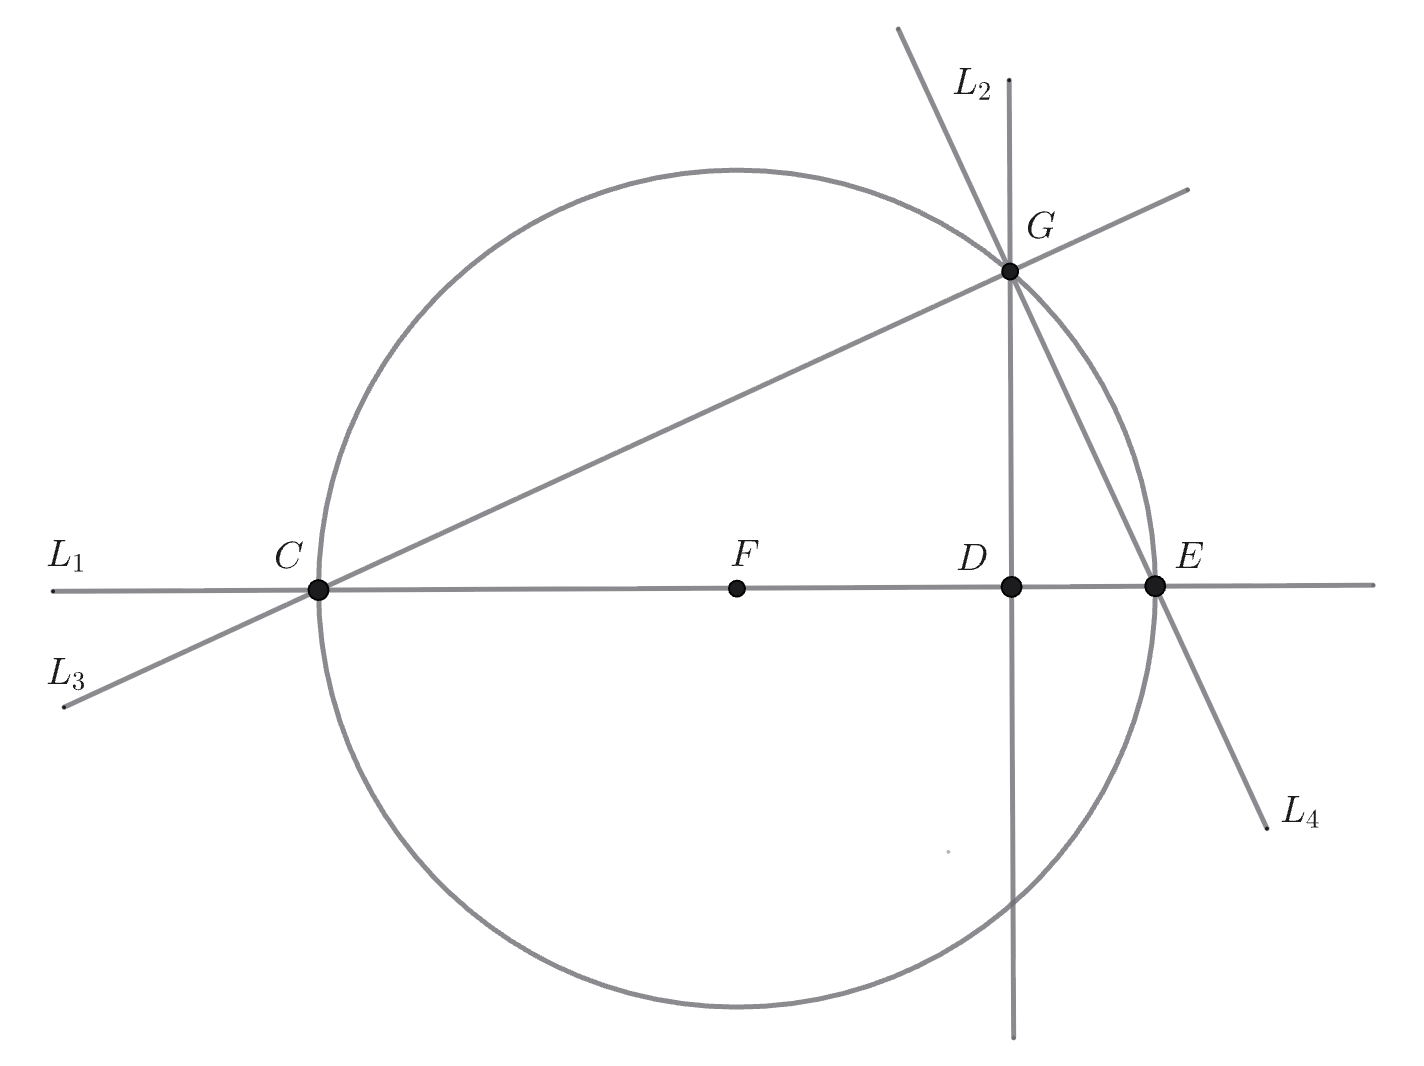
\includegraphics[scale=0.38]{pics/PropD.png}
    \caption{Proposition D}
\end{figure}

Combining propositions A, B, C and D, we can construct very complicated numbers such as $\sqrt{1 + \sqrt{2}}$ or $\sqrt{\sqrt{2} + \sqrt{3.5}}$. Let's now use the proof of these propositions to actually construct such a number. More precisely, let's construct $\sqrt{1 + \sqrt{2}}$ for example.

First, let's construct $\sqrt{2}$. To do this, let's extend the unit segment $AB$ into the straight line $L_1$ (Figure 8) (Axiom 2). Next, construct the straight line $L_2$ that passes through $A$ and that is perpendicular to $L_1$ (Proposition I.11), and construct the circle $\mathcal{C}_1$ with center $A$ and with radius $AB = 1$. Define the point $C$ as the lower point of intersection between $\mathcal{C}_1$ and $L_2$. By construction of $L_2$, then angle $BAC$ is a right angle and so $BAC$ is a right traingle. It follows by the Pythagorean Theorem (Proposition I.47) that $AB^2 + AC^2 = CB^2$. But we have $AB = AC = 1$ so $CB = \sqrt{2}$.

The next step is to construct $1 + \sqrt{2}$. To do this, simply construct the circle $\mathcal{C}_2$ with center $B$ and radius $BC = \sqrt{2}$ (Axiom 3) and define $D$ as the right-most point of intersection between $\mathcal{C}_2$ and $L_1$. By construction, $BD = BC = \sqrt{2}$ and so the segment $AD$ has length $1 + \sqrt{2}$.

The final step is to construct $\sqrt{1 + \sqrt{2}}$. Since we already constructed $1 + \sqrt{2}$, then we simply need to reproduce the construction in the proof of Proposition D. To do this, we need to construct a circle with center on $L_1$ such that the diamater has length $AD + 1 = 2 + \sqrt{2}$. To do this, construct the midpoint $E$ of the segment $BD$ (Proposition I.10) and construct the circle $\mathcal{C}_3$ with center $E$ and radius $AE$ (Axiom 3). Define $F$ as the right-most point of intersection between $\mathcal{C}_3$ and $L_1$. Then, by construction, we have
$$AF = 2AE = 2(AB) + 2BE = 2 + \sqrt{2}.$$
It follows that $\mathcal{C}_3$ is the circle we wanted. To finish the construction, simply construct the line $L_3$ that passes through $D$ and that is perpendicular to $L_1$ (Proposition I.11) and define $G$ as the point of intersection between $L_3$ and $\mathcal{C}_3$. By the proof of Proposition D, we have that the segment $DG$ has length $\sqrt{1 + \sqrt{2}}$.

\begin{figure}[h!]
    \centering
    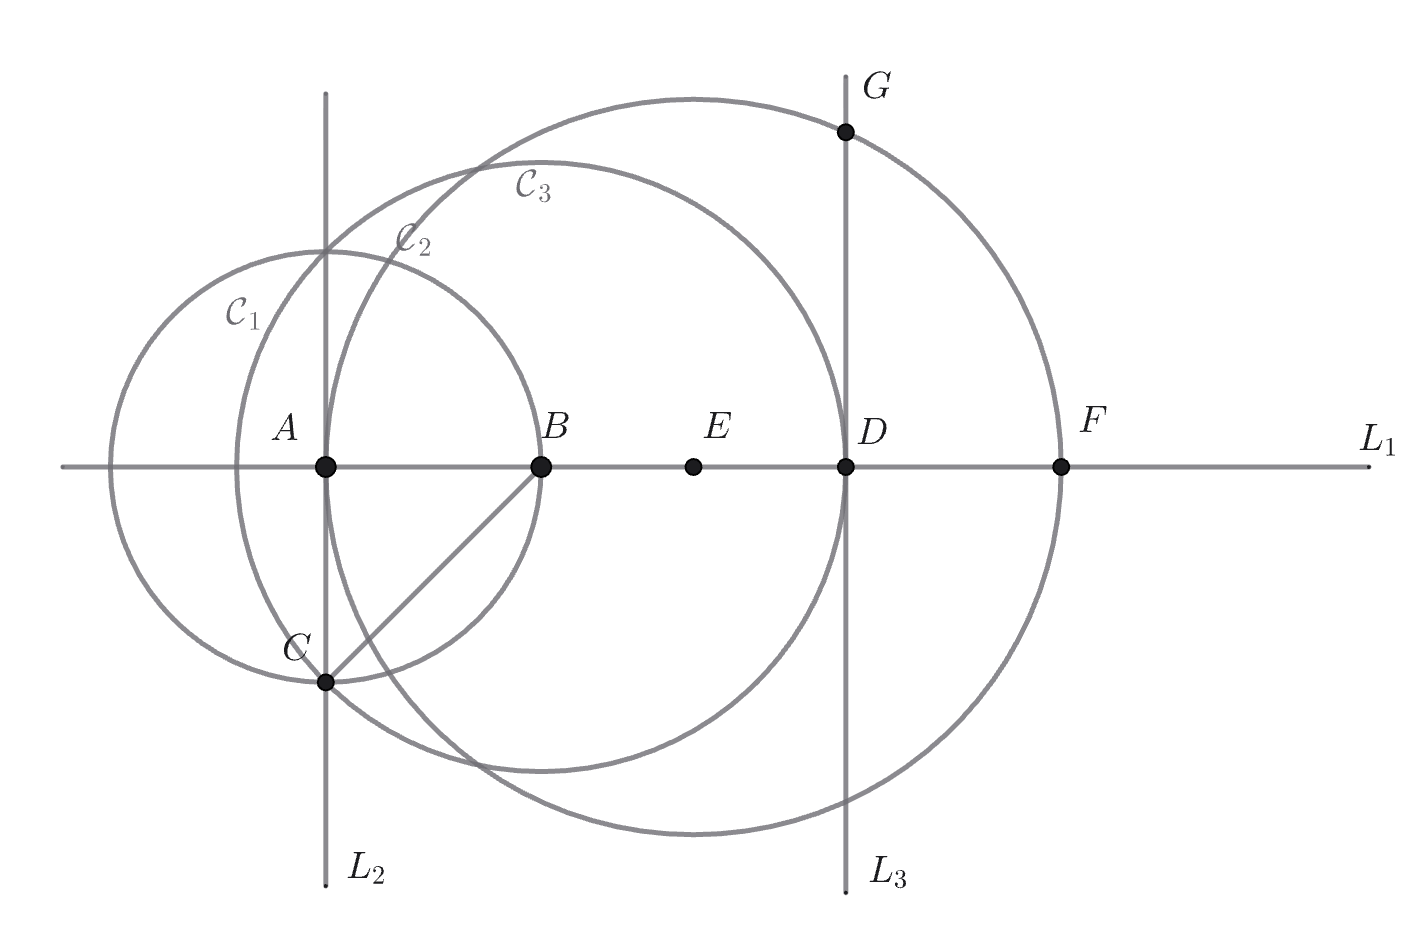
\includegraphics[scale=0.5]{pics/sqrt(2 + sqrt(2)).png}
    \caption{Construction of $\sqrt{1 + \sqrt{2}}$}
\end{figure}

\section*{Impossible Constructions}

The question still remains, is every number constructible ? Are addition, subtraction, multiplication, division and taking square roots the only operations we can apply to construcible numbers ? In a sense, the answer is yes. I will not prove it here but we indeed have the following characterization of constructible numbers: constructible numbers are precisely the numbers that can be obtained by applying successive addition, subtraction, multiplication, division, and taking square roots to rational numbers. 

Now that we have a better understanding of constructible numbers, lets answer this last question : are every positive real numbers constructible ? To answer it, we will have to define some terminology.

\begin{definition}[Algebraic and Transcendental Numbers]
    A real number is said to be \textit{algebraic} if it is a root of a polynomial with integer coefficients. If a number is not algebraic, we call it \textit{transcendental}.
\end{definition}

\noindent For example, the number $\sqrt{2}$ is algebraic since it is a root of the polynomial $x^2 - 2$. Similarly, any rational number $a/b$ is algebraic since it is a root of the polynomial $ax - b$. What about the number $\sqrt{1 + \sqrt{2}}$ which we constructed earlier, is it algebraic ? The answer is yes, and to prove it, let $a = \sqrt{1 + \sqrt{2}}$, then $a^2 = 1 + \sqrt{2}$. Equivalently, $a^2 - 1 = \sqrt{2}$. Squaring both sides gives us $(a^2 - 1)^2 = 2$ and so we get
$$a^4 - 2a^2 + 3 = 0.$$
Therefore, $\sqrt{1 + \sqrt{2}}$ is algebraic since it is a root of the polynomial $x^4 - 2x^2 + 3$. This motivates the following Theorem:

\begin{theorem*}
    Every constructible number is algebraic.
\end{theorem*}

\noindent The proof of this theorem requires some notions of Field Theory that would take us out of the scope of this document. The proof follows directly from the characterization of constructible that is mentioned above. If you are familiar with fields, I can show you the proof or give you some good resources for the proof of this theorem. A direct corollary to this theorem is the following:

\begin{corollary}
    Every transcendental number is not constructible.
\end{corollary}

\noindent The question now becomes: is it possible to find a positive transcendental number ? The answer is yes. Even more than that, the mathematician Georg Cantor proved in the late 1800's that there are more transcendental numbers than algebraic numbers. In the following decades, it was shown for example that both $\pi$ or $e$ (Euler's constant) are transcendental. Therefore, yes, $\pi$ is an example of a non-constructible positive real number, and so not every positive real number is constructible. \\

But the fact that $\pi$ is not construcible is actually of great importance because it also gives an answer to a very old problem in Euclidean Geometry : is it possible to \textit{square the circle}. In modern terms, given a circle, is it possible to construct a square which area is equal to the area of the circle ? We can now show that this is impossible. \\

\begin{theorem*}
    Given a constructible number $c$, it is impossible to construct a square which has the same area as the circle of radius $c$.
\end{theorem*}

\begin{proof}
    By contradiction, suppose that given a construcible number $c$, we can construct a square with the same area as the circle of radius $c$. We knwow that the circle (and so the square) must have area $\pi c^2$. Since the square is construcible, then its sides (which are segments) must be construcible as well. But since the area of the circle is $\pi c^2$, then its sides must have length $\sqrt{\pi} \cdot c$. Since the sides are construcible, then $\sqrt{\pi} \cdot c$ is a construcible number. By Proposition C, $\sqrt{\pi} \cdot c / c = \sqrt{\pi}$ is constructible. By Proposition B, $\sqrt{\pi} \cdot \sqrt{\pi} = \pi$ is construcible. This is in contradiction with the fact that $\pi$ is transcendental.
\end{proof}

The same kind of argument lets us prove that a lot of such constructions are impossible but again, it would take us far from the original goal of this document and it requires some more advanced tools. If you have any question regarding the content of this document, send me an email or ask me the question during the Tutorials.

\end{document}